\documentclass[11pt]{article}

\usepackage[margin=1in]{geometry}
\usepackage[T1]{fontenc}
\usepackage[utf8]{inputenc}
\usepackage{amsmath}
\usepackage{amssymb}
\usepackage{booktabs}
\usepackage{enumitem}
\usepackage{microtype}
\usepackage[numbers,sort&compress]{natbib}
\usepackage{pgfplots}
\usepackage{xcolor}
\usepackage{hyperref}

\pgfplotsset{compat=1.18}
\hypersetup{
  colorlinks=true,
  linkcolor=blue!50!black,
  citecolor=blue!50!black,
  urlcolor=blue!50!black
}

\newcommand{\code}[1]{\texttt{#1}}
\newcommand{\artifact}[1]{\path{#1}}
\newcommand{\modelname}{CodeLeWM}
\newcommand{\subA}{Substrate A}
\newcommand{\subB}{Substrate B}

\title{The Substrate Is the Bottleneck:\\
  A JEPA-style Code World Model on Code Edits and Program Execution}
\author{
  Abdelhamid Bakhta\\
  StarkWare\\
  \url{https://github.com/AbdelStark/CodeLeWM}
}
\date{Draft of June 1, 2026}

\begin{document}
\maketitle

\begin{abstract}
Joint-embedding predictive architectures (JEPAs) learn by predicting future
latent states rather than reconstructing observations. We ask whether a
JEPA-style latent-transition recipe can learn useful dynamics over code. In
\modelname{}, the answer depends strongly on the substrate.
Commit-message-conditioned Python edits over CommitPackFT-style data fail
across four scaled
Hugging Face Jobs runs: headline retrieval loses to the no-action baseline,
mutation surprise is chance-level, and the v0.2 action-swap run collapses to an
effective-rank ratio of 0.016. We then pivot the same model family and objective
registry to input-conditioned execution triples,
\((\mathrm{code}, \mathrm{input}) \mapsto \mathrm{output}\), produced by a
deterministic sandboxed Python executor. Across two v0.6 execution-substrate
seeds, the no-action margin flips from -0.77 to +1.24, SIGReg drops by about
\(1200\times\), and the predicted-latent effective-rank ratio reaches 0.47.
Evaluation on verified artifacts adds a narrow positive result: execution-pack
retrieval beats no-action by +61.4 Recall@1 points and +65.9 MRR points on
average, and semantic surprise decoy score gates reach AUC 1.0 on all
configured decoy categories. The result is partial, not a broad code-generation
or broad semantic-surprise claim: latent probes remain blocked by lexical
controls, crash prediction is not evaluable, and HumanEval/MBPP-Plus reranking
is not yet scored. The main lesson is that
substrate signal quality dominates objective tuning.
\end{abstract}

\section{Introduction}

JEPA-style world models replace pixel or token reconstruction with prediction
in a learned latent space. In images and video, this idea has produced
self-supervised representations that avoid direct generative decoding while
still learning useful structure \citep{assran2023selfsupervisedlearningimagesjointembedding,bardes2024revisitingfeaturepredictionlearning}.
LeWorldModel extends the same latent-prediction view to end-to-end visual
world models trained from pixels and actions \citep{maes2026leworldmodelstableendtoendjointembedding}.
Code is an intentionally hostile domain for that recipe. It is discrete,
structured, sparse, and semantically brittle: one token can change behavior
while large textual edits can be inert. The question is not just whether a JEPA
objective can be ported to code, but which code substrate gives the objective
enough signal to learn anything.

We study this question through a negative-to-positive substrate comparison in
\modelname, a latent world model for Python code transitions. In both settings,
the model predicts the latent of an after-state from the latent of a before-state
and an action:
\begin{equation}
  \hat z_{\mathrm{after}} =
  P(E(s_{\mathrm{before}}), A(a)).
\end{equation}
Both settings share the 256-dimensional transition contract, module family, and
objective registry. This is not a perfect ablation: the v0.6 execution runner
uses a substrate-specific loader, schedule, optimizer setting, and action-fusion
surface. The comparison is therefore a substrate-pivot claim inside one
implementation, not proof that every other variable is identical.

\subA{} treats a transition as a commit-message-conditioned code edit: before
code plus a commit message maps to after code. It is attractive because it
resembles the product surface of a patch scorer, but it has three structural
problems. First,
\(\mathrm{after} \approx \mathrm{before}\) is often a strong prior. Second,
commit messages are noisy, underspecified actions. Third, commits are often
multi-purpose, so no single canonical action-conditioned transformation exists.
The scaled evidence confirms the diagnosis. Four public runs all fail the
headline retrieval comparison against no-action; the strongest v0.2 run reports
an effective-rank ratio of 0.016, chance-level mutation surprise AUC 0.501, and
latent probes beaten by lexical or metadata controls.

\subB{} keeps the latent-transition contract but changes the world. It treats a
transition as a deterministic execution triple:
\((\mathrm{code}, \mathrm{input}) \mapsto \mathrm{output}\). Here the output is
not a near-copy of the code, the input is a precise typed action, and each row is
single-purpose. The v0.6 execution-substrate run inverts the failures above:
two training seeds reach effective-rank ratios of 0.467 and 0.477, the
no-action margin becomes strongly positive, and the execution-pack retrieval
gate beats no-action by more than 60 absolute Recall@1 points.

The contribution is deliberately scoped:
\begin{enumerate}[leftmargin=1.5em]
  \item A reproducible JEPA-style latent-transition recipe for code transitions,
  with manifest-backed data, checkpoints, and eval reports.
  \item A negative result on commit-message-conditioned code edits,
  showing that objective tweaks do not rescue a low-signal substrate.
  \item A partial-positive execution-substrate result under the same model
  family: non-collapse, action use, execution-pack retrieval, and
  semantic-decoy surprise score diagnostics pass across two seeds, while the
  broad semantic-surprise claim gate remains closed.
  \item An explicit claim boundary: the result is not a code generator, not a
  general semantic-axis result, and not yet HumanEval/MBPP-Plus reranking
  evidence.
\end{enumerate}

\section{Related Work}

\paragraph{Joint-embedding predictive architectures.}
I-JEPA predicts target image-block embeddings from context embeddings without
pixel reconstruction \citep{assran2023selfsupervisedlearningimagesjointembedding}.
V-JEPA extends this idea to video feature prediction
\citep{bardes2024revisitingfeaturepredictionlearning}. LeWorldModel uses a
latent prediction model for action-conditioned visual dynamics from pixels
\citep{maes2026leworldmodelstableendtoendjointembedding}. Our work preserves
the same core contract but changes the domain to code and compares two
substrates within one objective registry.

\paragraph{Anti-collapse regularization.}
The central technical risk in latent predictive models is collapse: a constant
encoder can make prediction losses appear small. VICReg and Barlow Twins add
variance, covariance, and redundancy-reduction constraints to self-supervised
learning \citep{bardes2022vicregvarianceinvariancecovarianceregularizationselfsupervised,zbontar2021barlowtwinsselfsupervisedlearning}.
LeJEPA and LeWorldModel study SIGReg-style regularization for stable
joint-embedding learning \citep{balestriero2025lejepaprovablescalableselfsupervised,maes2026leworldmodelstableendtoendjointembedding}.
\modelname{} inherits that anti-collapse emphasis and makes collapse gates a
first-class artifact.

\paragraph{Code representations and code generation benchmarks.}
Pretrained code models such as CodeBERT, GraphCodeBERT, UniXcoder, and CodeT5
learn representations or generation models from program text and natural
language \citep{feng2020codebertpretrainedmodelprogramming,guo2021graphcodebertpretrainingcoderepresentations,guo2022unixcoderunifiedcrossmodalpretraining,wang2021codet5identifierawareunifiedpretrained}.
CodeNet, MBPP, APPS, HumanEval, and EvalPlus/MBPP-Plus provide benchmark
substrates for program understanding, synthesis, and evaluation
\citep{puri2021codenetlargescaleaicode,austin2021programsynthesislargelanguage,hendrycks2021measuringcodingchallengecompetence,chen2021evaluatinglargelanguagemodels,liu2023codegeneratedchatgptreally}.
CodeT uses generated tests to rerank code generations
\citep{chen2022codetcodegenerationgenerated}. \modelname{} is not a generator:
it is a local latent scorer/reranker that can be applied to candidate code or
execution completions once labeled candidate artifacts exist.

\paragraph{Execution-aware program modeling.}
Execution has long been used as a supervised signal for neural program models,
from synthetic program evaluation to source-code pretraining with execution
traces \citep{zaremba2015learningexecute,ding2023tracedexecutionawarepretrainingsource}.
Recent execution-tuning work also studies models trained on program traces for
output prediction and execution reasoning
\citep{armengolestape2025iexecuteiunderstand}. \modelname{} differs in two
ways: it predicts latent next-state embeddings rather than emitting traces, and
its claim gate compares a commit-edit substrate against an execution substrate
under one artifact discipline.

\section{Model and Objective}

Both substrates use the same transition-model contract. A state encoder \(E\)
maps a bounded token capsule to \(z \in \mathbb{R}^{256}\). An action encoder \(A\)
maps either a commit message or an input representation to an action embedding.
A predictor \(P\) maps \((z_{\mathrm{before}}, A(a))\) to
\(\hat z_{\mathrm{after}}\). The training loss is
\begin{equation}
  \mathcal{L} =
  \|P(E(s_b), A(a)) - E(s_a)\|_2^2
  + \lambda_{\mathrm{sig}}\mathcal{L}_{\mathrm{SIGReg}}
  + \lambda_{\mathrm{swap}}\mathcal{L}_{\mathrm{swap}}
  + \lambda_{\mathrm{inv}}\mathcal{L}_{\mathrm{inv}}.
\end{equation}
The prediction term optimizes latent transition accuracy. SIGReg discourages
collapse. The action-swap term penalizes predictions under mismatched actions,
and the inverse-action term asks the model to preserve action information in the
latent transition. The closest \subA{} comparand, the v0.2 action-swap run, and
the v0.6 execution runs both enable this objective family. Their weights and
training configs differ, so we interpret the result as evidence for a substrate
pivot rather than as a single-factor architecture ablation.

\section{Substrates}

\paragraph{\subA: commit-message-conditioned edits.}
\subA{} uses permissively licensed CommitPackFT-style Python transitions. The
before-state and after-state are code capsules; the action is a natural-language
commit message. The v0.2 action-swap/inverse-action run packs 20,645
transitions with train/val/test counts 18,019/1,291/1,335. Its public report is
the v0.2 action-swap HF results report; the run artifact id is listed in the
claim audit.

\paragraph{\subB: input-conditioned execution.}
\subB{} uses deterministic Python execution records. The before-state is code,
the action is a serialized input, and the after-state is a serialized output.
The execution pack contains 1,605 records from CodeNet, MBPP, and APPS, with
HumanEval and MBPP-Plus held out for downstream evaluation. Candidate source
code is treated as untrusted input; sandbox execution is a data-build or
operator-labeling step, not a model-training or model-scoring step. The v0.6
pack id is \code{codelewm-execution-pack-20260528T102625Z}; the report is
\artifact{docs/benchmark/EXECUTION_V0_6_RESULTS_2026-05-30.md}.

\section{Experimental Protocol}

All quantitative claims in this draft trace to checked-in benchmark reports or
schema-versioned artifacts. For \subA{}, we use the v0.2 downloaded-artifact
verification report. For \subB{}, we use two HF Jobs training seeds, 42 and
1729, each trained to 50k steps on \code{a10g-small}. The \#305 eval pass reruns
the downloaded checkpoints through JSONL execution-pack eval surfaces:
execution retrieval, semantic-decoy surprise, latent probes, and crash
prediction. The committed eval tree is \artifact{docs/benchmark/v0_6/}; the
same tree is mirrored to the HF dataset repo at the commit recorded in the
claim audit, with the #322 semantic-surprise rerun recorded locally.

\section{Results}

\subsection{Training dynamics and non-collapse}

The training-time substrate-pivot claim passes on \subB{} and fails on \subA{}.
\subA{} v0.2 reaches an effective-rank ratio of only 0.016. \subB{} reaches
0.467 and 0.477 on seeds 42 and 1729, above the configured 0.20 gate.
Figure~\ref{fig:rank} shows the v0.6 predicted-latent effective-rank ratio over
training.

\begin{figure}[t]
\centering
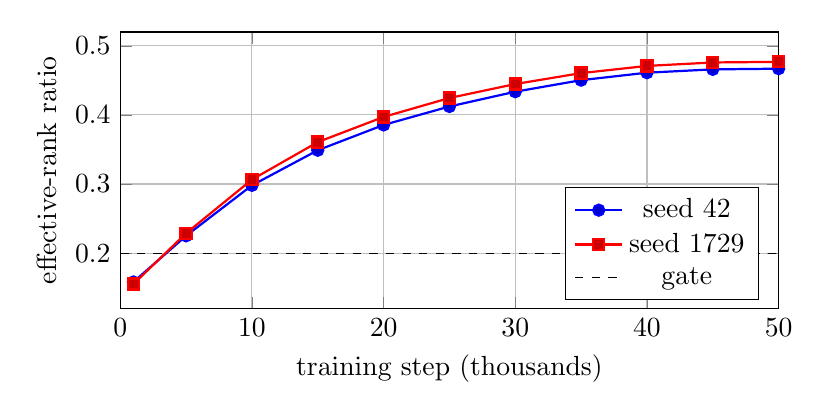
\begin{tikzpicture}
\begin{axis}[
  width=0.82\linewidth,
  height=0.42\linewidth,
  xlabel={training step (thousands)},
  ylabel={effective-rank ratio},
  ymin=0.12,
  ymax=0.52,
  xmin=0,
  xmax=50,
  grid=both,
  legend pos=south east
]
\addplot+[mark=*, thick] coordinates {
  (1,0.1583) (5,0.2251) (10,0.2981) (15,0.3489) (20,0.3855)
  (25,0.4122) (30,0.4336) (35,0.4503) (40,0.4611) (45,0.4659) (50,0.4669)
};
\addlegendentry{seed 42}
\addplot+[mark=square*, thick] coordinates {
  (1,0.1553) (5,0.2288) (10,0.3064) (15,0.3607) (20,0.3971)
  (25,0.4245) (30,0.4447) (35,0.4605) (40,0.4709) (45,0.4759) (50,0.4768)
};
\addlegendentry{seed 1729}
\addplot+[black, dashed, mark=none] coordinates {(0,0.20) (50,0.20)};
\addlegendentry{gate}
\end{axis}
\end{tikzpicture}
\caption{v0.6 predicted-latent effective-rank ratio from the collapse
diagnostics report. Both seeds cross the 0.20 collapse gate early and finish
near 0.47.}
\label{fig:rank}
\end{figure}

The v0.6 no-action margin also flips sign quickly and remains positive in raw
training metrics (Figure~\ref{fig:margin}). The report-level final metrics
average to +1.2308 for seed 42 and +1.2434 for seed 1729.

\begin{figure}[t]
\centering
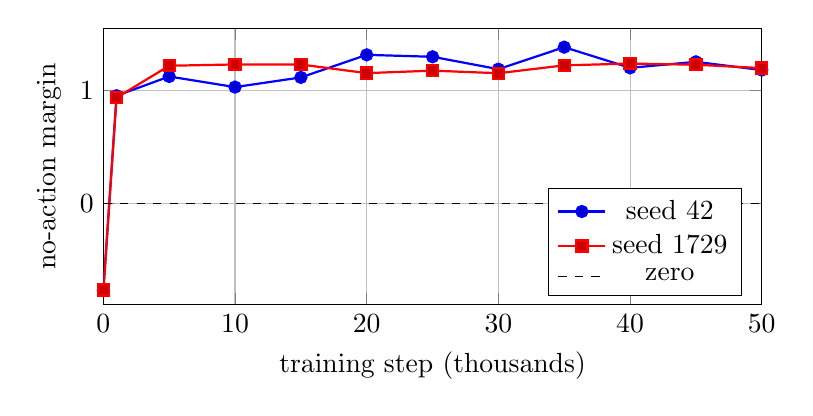
\begin{tikzpicture}
\begin{axis}[
  width=0.82\linewidth,
  height=0.42\linewidth,
  xlabel={training step (thousands)},
  ylabel={no-action margin},
  ymin=-0.9,
  ymax=1.55,
  xmin=0,
  xmax=50,
  grid=both,
  legend pos=south east
]
\addplot+[mark=*, thick] coordinates {
  (0.001,-0.7722) (1,0.9517) (5,1.1222) (10,1.0283) (15,1.1140)
  (20,1.3141) (25,1.2969) (30,1.1871) (35,1.3822) (40,1.1989)
  (45,1.2522) (50,1.1793)
};
\addlegendentry{seed 42}
\addplot+[mark=square*, thick] coordinates {
  (0.001,-0.7689) (1,0.9346) (5,1.2175) (10,1.2289) (15,1.2285)
  (20,1.1520) (25,1.1741) (30,1.1512) (35,1.2209) (40,1.2370)
  (45,1.2264) (50,1.1968)
};
\addlegendentry{seed 1729}
\addplot+[black, dashed, mark=none] coordinates {(0,0) (50,0)};
\addlegendentry{zero}
\end{axis}
\end{tikzpicture}
\caption{Raw v0.6 no-action margin training metric. Positive values mean the
action-conditioned prediction is closer to the target than the no-action
latent.}
\label{fig:margin}
\end{figure}

\begin{table}[t]
\centering
\caption{Headline training and collapse metrics from the v0.2 and v0.6
benchmark reports. Raw MSE values are diagnostic within a substrate and should
not be read as cross-substrate quality scores.}
\label{tab:training}
\begin{tabular}{lrrrr}
\toprule
Run & prediction MSE & SIGReg & no-action margin & effective-rank ratio \\
\midrule
v0.2 action-swap & 0.1494 & -- & -- & 0.0158 \\
v0.6 seed 42 & 0.00064 & 0.0364 & +1.2308 & 0.4669 \\
v0.6 seed 1729 & 0.00060 & 0.0348 & +1.2434 & 0.4768 \\
\bottomrule
\end{tabular}
\end{table}

\subsection{Retrieval}

Retrieval is the cleanest action-use measurement. For \subA{}, the model must
rank true after-states above hard negatives, but no-action remains stronger.
For \subB{}, the query is an execution record and the candidate set is 236
val/test outputs. Table~\ref{tab:retrieval} shows the contrast.

\begin{table}[t]
\centering
\caption{Retrieval comparison. Positive deltas mean the action-conditioned
model beats no-action.}
\label{tab:retrieval}
\begin{tabular}{llrrrr}
\toprule
Substrate & Run & Recall@1 & $\Delta$ vs no-action & MRR & $\Delta$ vs no-action \\
\midrule
A & \#138 & 0.371 & -0.088 & 0.473 & -0.073 \\
A & \#154 & 0.363 & -0.106 & 0.468 & -0.082 \\
A & \#159 & 0.597 & -0.053 & 0.675 & -0.034 \\
A & \#172 & 0.263 & -0.178 & 0.370 & -0.163 \\
B & v0.6 seed 42 & 0.657 & +0.619 & 0.767 & +0.663 \\
B & v0.6 seed 1729 & 0.648 & +0.610 & 0.759 & +0.655 \\
\bottomrule
\end{tabular}
\end{table}

Mean v0.6 Recall@1 is 0.6525 and mean MRR is 0.7628. Mean lift over
no-action is +0.6144 Recall@1 and +0.6588 MRR, with seed-to-seed spread below
one point. This supports a narrow execution-pack retrieval claim.

\subsection{Surprise and decoys}

\subA{} v0.2 mutation surprise is chance-level: mutation AUC 0.501. \subB{}
v0.6 semantic surprise reruns pass all configured numeric score gates
(Table~\ref{tab:surprise}). The caveat is important: same-problem-different
submission still has only six scored pairs after filtering, so the explicit
claim gate remains closed even though the broader semantic decoy pack contains
358 same-problem pairs across 68 problems.

\begin{table}[t]
\centering
\caption{v0.6 semantic surprise AUCs and count-gate status from the committed
per-seed surprise reruns.}
\label{tab:surprise}
\begin{tabular}{lrrrl}
\toprule
Run & mutation & same-code/different-input & same-problem/different-submission & claim gate \\
\midrule
v0.6 seed 42 & 1.000 / 236 & 1.000 / 352 & 1.000 / 6 & closed: $6<30$ \\
v0.6 seed 1729 & 1.000 / 236 & 1.000 / 352 & 1.000 / 6 & closed: $6<30$ \\
\bottomrule
\end{tabular}
\end{table}

\subsection{Latent probes, crash prediction, and reranking}

The broader downstream story is not positive. Only \code{output\_type} has
train/val/test labels for v0.6 latent probes. The latent view beats no-action
by 5.7 points on both seeds, but lexical controls remain stronger
(Table~\ref{tab:probe}). The report therefore closes the positive
representation claim gate.

\begin{table}[t]
\centering
\caption{v0.6 output-type latent-probe test accuracy.}
\label{tab:probe}
\begin{tabular}{lrrrr}
\toprule
Run & \(z_{\mathrm{pred}}\) & no-action & lexical & claim \\
\midrule
v0.6 seed 42 & 0.497 & 0.439 & 0.662 & blocked \\
v0.6 seed 1729 & 0.599 & 0.541 & 0.618 & blocked \\
\bottomrule
\end{tabular}
\end{table}

Crash prediction is not evaluable because both v0.6 val/test slices have
0 positives and 236 negatives. HumanEval/MBPP-Plus reranking is also not
scored: the sampler and
\artifact{codelewm.eval.completion_label.v1} contract exist, but full live
labeled-completion artifacts are not present. No HumanEval/MBPP-Plus pass@1
lift claim is allowed from the current evidence.

\section{Discussion}

The comparison supports one main explanation: the substrate is the bottleneck.
On commit-message-conditioned edits, the model family has a strong shortcut. A
no-action or identity-like prior is often correct, and the action text is too
vague to force a different latent prediction. Objective variants improve some
diagnostics but do not invert the headline gate.

Execution triples remove that shortcut. The output token distribution is
different from the code distribution; copying the code latent is structurally
wrong. The action is a deterministic value rather than a free-form commit
message. Each row is single-purpose and judge-verifiable. Under these
conditions, the execution objective produces non-collapsed latents and strong
execution-pack retrieval.

This does not mean the model understands programs in a broad sense. The probe
result is deliberately humbling: lexical features still beat the latent view on
the only evaluable semantic target. The surprise result is also limited by
generated decoys. The right conclusion is not that \modelname{} solves code
generation; it is that a JEPA-style latent transition model can learn an
action-conditioned execution substrate when the substrate supplies precise
state/action/next-state signal.

\section{Limitations}

\begin{itemize}[leftmargin=1.5em]
  \item The execution substrate is Python-only and stdlib-only under the current
  sandbox policy.
  \item The v0.6 result uses two training seeds. This is enough to check a
  large effect with small spread, but it is not a full variance study.
  \item The comparison is not a perfectly controlled ablation. The v0.6
  execution run changes the loader, optimizer schedule, effective batch size,
  and action-fusion surface while preserving the latent-transition model family
  and objective registry. The causal claim is therefore scoped to the observed
  substrate pivot, not to substrate as the only changed variable.
  \item HumanEval and MBPP-Plus reranking are not evaluated in the current
  artifact set. A live OpenRouter sampling and hidden-test labeling run is
  still required.
  \item Generated surprise decoys are useful diagnostics but not full
  adversarial semantic tests. The strengthened semantic pack adds 352
  same-code/different-input pairs, but the narrow same-problem/different
  submission category still has only six pairs.
  \item The paper compares substrates inside one implementation and objective
  registry. It does not claim superiority over large pretrained code models.
\end{itemize}

\section{Reproducibility and Artifacts}

The public artifact chain is intentionally part of the result. The code lives
at \url{https://github.com/AbdelStark/CodeLeWM}. \subA{} uses
\artifact{abdelstark/codelewm-public-shard},
\artifact{abdelstark/codelewm-transition-model}, and
\artifact{abdelstark/codelewm-runs}. \subB{} uses
\artifact{abdelstark/codelewm-execution-pack@v0.6.0} and the two seed-specific
v0.6 run artifacts in \artifact{abdelstark/codelewm-runs}. The \#305 eval
reports are committed under \artifact{docs/benchmark/v0_6/} and mirrored to
the HF dataset repo. Every published artifact is manifest-backed and
secret-scanned.

The claim audit for this draft is
\artifact{docs/papers/two_substrate_claim_audit.md}. The build command is:
\begin{verbatim}
scripts/build-two-substrate-paper
\end{verbatim}

\section{Conclusion}

The negative v0.2 result and partial-positive v0.6 result are not contradictory.
They are the point. A JEPA-style code world model does not become useful merely
because the objective includes prediction, anti-collapse regularization, and
action-contrastive terms. It needs a substrate where the action actually
constrains the next state. For code, commit-message-conditioned edits did not
provide that signal; deterministic execution triples did. The practical lesson
for future code-world-model work is simple: pick the substrate before picking
the architecture.

\bibliographystyle{plainnat}
\bibliography{two_substrate_references}

\end{document}
